\documentclass[portrait,final,a0paper,fontscale=0.277]{baposter}

\usepackage{calc}
\usepackage{graphicx}
\usepackage{amsmath}
\usepackage{amssymb}
\usepackage{relsize}
\usepackage{multirow}
\usepackage{rotating}
\usepackage{bm}
\usepackage{url}
   
\usepackage{graphicx}
\usepackage{multicol}
\usepackage{tabulary}
%\usepackage{times}
%\usepackage{helvet}
%\usepackage{bookman}
\usepackage{palatino}
\usepackage[utf8]{inputenc}
\usepackage[spanish]{babel}
\usepackage{booktabs}
\usepackage{tikz}
\usepackage{tkz-kiviat}
\usetikzlibrary{shapes,arrows,shadows}
%\usepackage[style=numeric,sorting=none,backend=biber]{biblatex}
%\addbibresource{../bibliography.bib}


\newcommand{\captionfont}{\footnotesize}

\graphicspath{{images/}{../images/}}
\usetikzlibrary{calc}

\newcommand{\SET}[1]  {\ensuremath{\mathcal{#1}}}
\newcommand{\MAT}[1]  {\ensuremath{\boldsymbol{#1}}}
\newcommand{\VEC}[1]  {\ensuremath{\boldsymbol{#1}}}
\newcommand{\Video}{\SET{V}}
\newcommand{\video}{\VEC{f}}
\newcommand{\track}{x}
\newcommand{\Track}{\SET T}
\newcommand{\LMs}{\SET L}
\newcommand{\lm}{l}
\newcommand{\PosE}{\SET P}
\newcommand{\posE}{\VEC p}
\newcommand{\negE}{\VEC n}
\newcommand{\NegE}{\SET N}
\newcommand{\Occluded}{\SET O}
\newcommand{\occluded}{o}

%%%%%%%%%%%%%%%%%%%%%%%%%%%%%%%%%%%%%%%%%%%%%%%%%%%%%%%%%%%%%%%%%%%%%%%%%%%%%%%%
%%%% Some math symbols used in the text
%%%%%%%%%%%%%%%%%%%%%%%%%%%%%%%%%%%%%%%%%%%%%%%%%%%%%%%%%%%%%%%%%%%%%%%%%%%%%%%%

%%%%%%%%%%%%%%%%%%%%%%%%%%%%%%%%%%%%%%%%%%%%%%%%%%%%%%%%%%%%%%%%%%%%%%%%%%%%%%%%
% Multicol Settings
%%%%%%%%%%%%%%%%%%%%%%%%%%%%%%%%%%%%%%%%%%%%%%%%%%%%%%%%%%%%%%%%%%%%%%%%%%%%%%%%
\setlength{\columnsep}{1.5em}
\setlength{\columnseprule}{0mm}

%%%%%%%%%%%%%%%%%%%%%%%%%%%%%%%%%%%%%%%%%%%%%%%%%%%%%%%%%%%%%%%%%%%%%%%%%%%%%%%%
% Save space in lists. Use this after the opening of the list
%%%%%%%%%%%%%%%%%%%%%%%%%%%%%%%%%%%%%%%%%%%%%%%%%%%%%%%%%%%%%%%%%%%%%%%%%%%%%%%%
\newcommand{\compresslist}{%
\setlength{\itemsep}{1pt}%
\setlength{\parskip}{0pt}%
\setlength{\parsep}{0pt}%
}
\newcommand{\tabitem}{~~\llap{\textbullet}~~}
\setlength{\leftmargini}{1em}

\newcommand{\pin}[2]{{\textbf{#2}}}
%%%%%%%%%%%%%%%%%%%%%%%%%%%%%%%%%%%%%%%%%%%%%%%%%%%%%%%%%%%%%%%%%%%%%%%%%%%%%%
%%% Begin of Document
%%%%%%%%%%%%%%%%%%%%%%%%%%%%%%%%%%%%%%%%%%%%%%%%%%%%%%%%%%%%%%%%%%%%%%%%%%%%%%
\begin{document}

%%%%%%%%%%%%%%%%%%%%%%%%%%%%%%%%%%%%%%%%%%%%%%%%%%%%%%%%%%%%%%%%%%%%%%%%%%%%%%
%%% Here starts the poster
%%%---------------------------------------------------------------------------
%%% Format it to your taste with the options
%%%%%%%%%%%%%%%%%%%%%%%%%%%%%%%%%%%%%%%%%%%%%%%%%%%%%%%%%%%%%%%%%%%%%%%%%%%%%%
% Define some colors

%\definecolor{lightblue}{cmyk}{0.83,0.24,0,0.12}
\definecolor{lightblue}{rgb}{0.145,0.6666,1}

% Draw a video
\newlength{\FSZ}
\newcommand{\drawvideo}[3]{% [0 0.25 0.5 0.75 1 1.25 1.5]
   \noindent\pgfmathsetlength{\FSZ}{\linewidth/#2}
   \begin{tikzpicture}[outer sep=0pt,inner sep=0pt,x=\FSZ,y=\FSZ]
   \draw[color=lightblue!50!black] (0,0) node[outer sep=0pt,inner sep=0pt,text width=\linewidth,minimum height=0] (video) {\noindent#3};
   \path [fill=lightblue!50!black,line width=0pt] 
     (video.north west) rectangle ([yshift=\FSZ] video.north east) 
    \foreach \x in {1,2,...,#2} {
      {[rounded corners=0.6] ($(video.north west)+(-0.7,0.8)+(\x,0)$) rectangle +(0.4,-0.6)}
    }
;
   \path [fill=lightblue!50!black,line width=0pt] 
     ([yshift=-1\FSZ] video.south west) rectangle (video.south east) 
    \foreach \x in {1,2,...,#2} {
      {[rounded corners=0.6] ($(video.south west)+(-0.7,-0.2)+(\x,0)$) rectangle +(0.4,-0.6)}
    }
;
   \foreach \x in {1,...,#1} {
     \draw[color=lightblue!50!black] ([xshift=\x\linewidth/#1] video.north west) -- ([xshift=\x\linewidth/#1] video.south west);
   }
   \foreach \x in {0,#1} {
     \draw[color=lightblue!50!black] ([xshift=\x\linewidth/#1,yshift=1\FSZ] video.north west) -- ([xshift=\x\linewidth/#1,yshift=-1\FSZ] video.south west);
   }
   \end{tikzpicture}
}

\hyphenation{resolution occlusions}

%%
\begin{poster}%
  % Poster Options
  {
  % Show grid to help with alignment
  grid=false,
  % Column spacing
  colspacing=1em,
  % Color style
  bgColorOne=white,
  bgColorTwo=white,
  borderColor=lightblue,
  headerColorOne=black,
  headerColorTwo=lightblue,
  headerFontColor=white,
  boxColorOne=white,
  boxColorTwo=lightblue,
  % Format of textbox
  textborder=roundedleft,
  % Format of text header
  eyecatcher=true,
  headerborder=closed,
  headerheight=0.12\textheight,
%  textfont=\sc, An example of changing the text font
  headershape=roundedright,
  headershade=shadelr,
  headerfont=\Large\bf\textsc, %Sans Serif
  textfont={\setlength{\parindent}{1.5em}},
  boxshade=plain,
%  background=shade-tb,
  background=plain,
  linewidth=2pt
  }
  % Eye Catcher
  {
\includegraphics[height=7em]{imagenes/logouna.png}} 
  % Title
  {\bf\textsc{Juegos serios como apoyo a la formación de
          profesionales:\hspace{5cm} Una aplicación al área de enfermería}\vspace{0.5em}}
  % Authors
  {\textsc{Mirta González y Arturo Volpe}}
  % University logo
  {% The makebox allows the title to flow into the logo, this is a hack because of the L shaped logo.
    
\includegraphics[height=9em]{../util/logo.pdf}
  }

%%%%%%%%%%%%%%%%%%%%%%%%%%%%%%%%%%%%%%%%%%%%%%%%%%%%%%%%%%%%%%%%%%%%%%%%%%%%%%
%%% Now define the boxes that make up the poster
%%%---------------------------------------------------------------------------
%%% Each box has a name and can be placed absolutely or relatively.
%%% The only inconvenience is that you can only specify a relative position 
%%% towards an already declared box. So if you have a box attached to the 
%%% bottom, one to the top and a third one which should be in between, you 
%%% have to specify the top and bottom boxes before you specify the middle 
%%% box.
%%%%%%%%%%%%%%%%%%%%%%%%%%%%%%%%%%%%%%%%%%%%%%%%%%%%%%%%%%%%%%%%%%%%%%%%%%%%%%
    %
    % A coloured circle useful as a bullet with an adjustably strong filling
    \newcommand{\colouredcircle}{%
      \tikz{\useasboundingbox (-0.2em,-0.32em) rectangle(0.2em,0.32em);
          \draw[draw=black,fill=lightblue,line width=0.03em] (0,0) circle(0.18em);}\-\ }

%%%%%%%%%%%%%%%%%%%%%%%%%%%%%%%%%%%%%%%%%%%%%%%%%%%%%%%%%%%%%%%%%%%%%%%%%%%%%%
  \headerbox{Introducción}{name=introduccion,column=0,row=0}{
%%%%%%%%%%%%%%%%%%%%%%%%%%%%%%%%%%%%%%%%%%%%%%%%%%%%%%%%%%%%%%%%%%%%%%%%%%%%%%
    El rol de las Tecnologías de la Información y la Comunicación (TIC) en la
    educación es, tradicionalmente, un mecanismo más para transmitir el
    conocimiento del maestro al alumno. Actualmente las nuevas corrientes
    pedagógicas requieren que su rol en la educación sea más activo dentro  del
    proceso de aprendizaje, ayudando incluso al alumno en la construcción del
    conocimiento. 
  	
  	Este trabajo se centra en los juegos serios, que se definen como videojuegos 
	que tienen un objetivo pedagógico específico, sin descuidar los aspectos  
	lúdicos ni el involucramiento del usuario\cite{abt1987serious}.
   \vspace{0.3em}
 }

%%%%%%%%%%%%%%%%%%%%%%%%%%%%%%%%%%%%%%%%%%%%%%%%%%%%%%%%%%%%%%%%%%%%%%%%%%%%%%
  \headerbox{Objetivo General}{name=objetivo,column=0,below=introduccion}{%
%%%%%%%%%%%%%%%%%%%%%%%%%%%%%%%%%%%%%%%%%%%%%%%%%%%%%%%%%%%%%%%%%%%%%%%%%%%%%%
   Identificar y valorar los factores pedagógicos, de diseño, de implementación
   y de evaluación que influyen a la creación de herramientas educativas que
   utilizan las corrientes pedagógicas actuales apoyadas en las TIC,
   especialmente los juegos serios. 

   \vspace{0.3em}
  }



%%%%%%%%%%%%%%%%%%%%%%%%%%%%%%%%%%%%%%%%%%%%%%%%%%%%%%%%%%%%%%%%%%%%%%%%%%%%%%
  \headerbox{Motivación}{name=problema,column=0,below=objetivo}{%
%%%%%%%%%%%%%%%%%%%%%%%%%%%%%%%%%%%%%%%%%%%%%%%%%%%%%%%%%%%%%%%%%%%%%%%%%%%%%%
      %Este trabajo se centra en las problemáticas referentes al área de
%enfermería proponiendo una solución basada en las TIC. Se considera como
%campo de estudio al Instituto Doctor Andrés Barbero, cuyos estudiantes del %último año de la carrera de Licenciatura en Enfermería son tomados como %población objetivo.
\begin{itemize}
\item Los juegos serios son herramientas que ayudan al desarrollo del pensamiento 
	crítico, sus principales áreas de aplicación son la militar, la salud y la 
	empresarial
\item Los estudiantes de enfermería aprenden a través de la experimentación
    activa y reflexionando sobre su experiencia, los juegos serios son una
    herramienta ideal para este tipo de
    estudiantes\cite{humphreys2013developing}.
\item Los estudiantes de enfermería poseen poca disponibilidad de tiempo para
    actividades extras debido al tiempo que dedican a las prácticas, a las
    clases teóricas y al transporte\cite{iab:tesis_alumnos}.
\item La personalización de la enseñanza es difícil debido a la gran cantidad de
    alumnos\cite{iab:tesis_alumnos}.

%\item La mayoría los juegos serios ofrecen una experiencia muy guiada, %dificultando el desarrollo del pensamiento crítico y la toma 
%de decisiones.

\end{itemize}

%Uno de los principales inconvenientes de los estudiantes es la poca
%disponibilidad de tiempo que poseen\cite{iab:tesis_alumnos}, la difícil 
%personalización de la enseñanza en las prácticas\cite{iab:tesis_alumnos} y el %nerviosismo ante las primeras prácticas.

%Según~\cite{humphreys2013developing} los alumnos de enfermería son estudiantes
%divergentes, es decir aprenden a través de experimentación activa, e
%interiorizan el conocimiento reflexionando sobre la experiencia. Los juegos
%serios son una herramienta ideal para este tipo de
%estudiantes\cite{humphreys2013developing}. 
 \vspace{0.3em}
  }
    
  
%%%%%%%%%%%%%%%%%%%%%%%%%%%%%%%%%%%%%%%%%%%%%%%%%%%%%%%%%%%%%%%%%%%%%%%%%%%%%%
  \headerbox{Conclusiones}{name=conclusiones,column=0,below=problema, above=bottom}{%
%%%%%%%%%%%%%%%%%%%%%%%%%%%%%%%%%%%%%%%%%%%%%%%%%%%%%%%%%%%%%%%%%%%%%%%%%%%%%%
\begin{itemize}

%\item La solución es válida como herramienta educativa de apoyo a los
    %estudiantes de enfermería, dándoles la posibilidad de probar sus
    %conocimientos en cualquier lugar y momento.

%\item  No se considera que se aprenda mejor con respecto otros métodos, sino
    %que, ya sea por motivación, interés o curiosidad,
    %puede ayudar en el proceso de enseñanza-aprendizaje dándole un rol más
    %activo a las TIC. 

%\item Los datos muestran una mejoría del $10\%$ entre los alumnos que utilizaron
%    y los que no utilizaron la solución. 
    
%\item Las correlaciones indican que los usuarios que más tiempo dedicaron a la solución,
%    mejor rendimiento obtuvieron en los procedimientos. Además aquellos
%    que mejor puntaje alcanzaron en la solución, mejor nota obtuvieron en la prueba
%    de conocimiento.
    
\item La solución obtuvo una aceptación positiva en todos los factores
    estudiados.
\item Los estudiantes consideraron a la solución como una herramienta útil para
    el apoyo de sus clases teóricas, prácticas de laboratorio y prácticas de
    campo.
\item La utilización de la solución se dio mayormente en horarios
    extracurriculares, acentuándose así la importancia de la movilidad proveída.
%\item Los usuarios que utilizaron más tiempo la solución obtuvieron mejores
%    puntuaciones en el juego.
\item Los usuarios con mejor puntuación en el juego obtuvieron mejor nota en la
    prueba de conocimiento.

\end{itemize}

}
 
%%%%%%%%%%%%%%%%%%%%%%%%%%%%%%%%%%%%%%%%%%%%%%%%%%%%%%%%%%%%%%%%%%%%%%%%%%%%%%
\headerbox{Solución propuesta}{name=solucion,column=1,span=2,row=0}{%
%%%%%%%%%%%%%%%%%%%%%%%%%%%%%%%%%%%%%%%%%%%%%%%%%%%%%%%%%%%%%%%%%%%%%%%%%%%%%%

Se diseña y desarrolla un Juego Serio para dispositivos móviles llamado
\textit{eTesãi}, el cual ofrece a los estudiantes de enfermería un medio para
realizar procedimientos de enfermería y cuyo objetivo es servir como herramienta
de apoyo al aprendizaje. En la figura se observan los componentes de la solución.
%,y las herramientas utilizadas para su desarrollo.

\begin{center}
    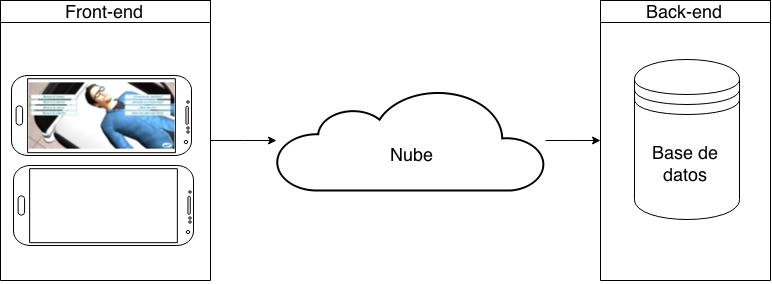
\includegraphics[scale=0.3]{../tecnologias/images/full.png}
\end{center}
\setlength{\columnsep}{1pt}
\begin{multicols}{2}
    \begin{itemize}

    \item \textbf{Front-end:} es una aplicación \textit{Android}, la cual es
        utilizada por los estudiantes para realizar procedimientos
        de enfermería. 
        
        Las escenas presentadas corresponden a los siguientes
        procedimientos:
        
        \begin{itemize}
        
        \item \textbf{Venopunción}
      
        El objetivo principal de este procedimiento es extraer muestras de sangre 
        del paciente para su análisis en un laboratorio.
    	\begin{center}
    		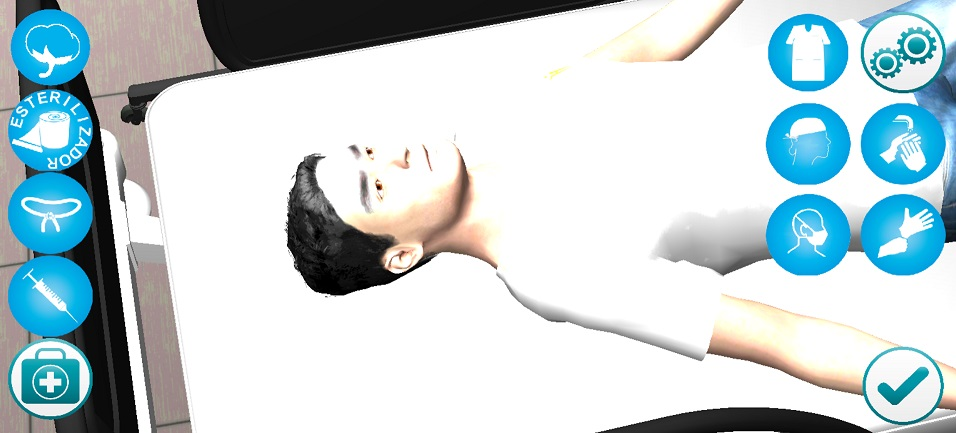
\includegraphics[width=4cm]{../solucion/images/hemocultivo_gui.jpg}
    	\end{center}
		
        \item \textbf{Valoración de la escala de Glasgow}
	
		El objetivo principal de este procedimiento es diagnosticar el estado de 
		conciencia de un paciente en estado crítico, utilizando la escala 
		de \textit{Glasgow}
		\begin{center}
		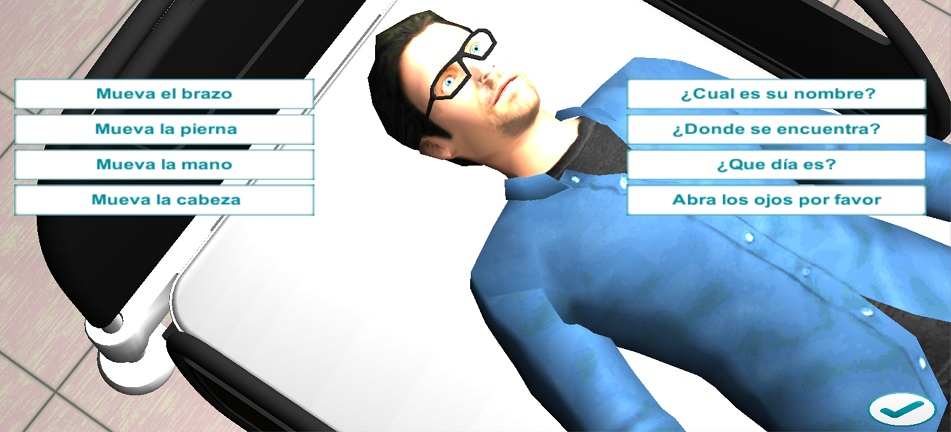
\includegraphics[width=4cm]{../solucion/images/glasgow_comandos_voz.jpg}
		\end{center}
		\end{itemize}
		
    \item \textbf{Back-end:} los registros de uso del \textit{front-end} son
        almacenados bajo demanda en un servidor \textit{back-end}, el cual se
        encarga de asociar los registros con los alumnos y almacenarlos de
        manera persistente.
    \end{itemize}
\end{multicols}

 \vspace{-0.6em}
}

%%%%%%%%%%%%%%%%%%%%%%%%%%%%%%%%%%%%%%%%%%%%%%%%%%%%%%%%%%%%%%%%%%%%%%%%%%%%%%
  \headerbox{Resultados obtenidos}{name=resultados,column=1, span=2, row=0,below=solucion}{
%%%%%%%%%%%%%%%%%%%%%%%%%%%%%%%%%%%%%%%%%%%%%%%%%%%%%%%%%%%%%%%%%%%%%%%%%%%%%%
\begin{multicols}{2}
\textbf{Metodología utilizada}
\begin{center}
\scriptsize 
\begin{tabular}{ll}
\toprule
\textbf{Variables}        & Aceptación, uso y conocimiento\\
\midrule
\textbf{Participantes}    & \shortstack{Alumnos del 4to año de Enfermería \\del Instituto Dr. Andrés Barbero}\\
\midrule
\textbf{Fases y duración} & \tabitem Instalación de la aplicación. \textbf{2 min} \\
					      & \tabitem Explicación de la GUI. \textbf{10 min} \\
					      & \tabitem Utilización de la aplicación. \textbf{20 días}\\
					      & \tabitem Encuesta de apreciación. \textbf{20 min} \\
					      & \tabitem Encuesta sobre conocimiento. \textbf{20 min} \\
					      & \tabitem Recopilación de datos  \\


\bottomrule
\end{tabular}
\end{center}

\textbf{Encuesta de apreciación}
\begin{center}

\scriptsize 
\begin{tabular}{lc}
\toprule
Factores                 & Promedio encuesta  \\
\midrule
Motivación               & De acuerdo    			\\
Facilidad de exploración & De acuerdo               \\
Sensación de Inmersión   & De acuerdo               \\
Pedagogía                & De acuerdo               \\
Representación           & Parcialmente de acuerdo  \\
Retroalimentación        & Parcialmente de acuerdo  \\
Utilidad                 & De acuerdo               \\
\bottomrule
\end{tabular}

%\tiny
%\begin{tikzpicture}[label distance=.15cm]
%    \tkzKiviatDiagram[scale=.35,%
%                            lattice=9,
%                            %step=10,
%                            ]
%                        {Motivación,
%                         Exploración,
%                        Inmersión,
%                         Pedagogía,
%                         Representación,
%                         Retroalimentación,
%                         Utilidad}
%     \tkzKiviatLine[thick,
%                        color=blue!25!white,
%                        mark=ball,
%                        ball color=blue,
%                        mark size=5pt,
%                        opacity=.2, 
%                        fill=blue!20](6.7,6.8,6.3,6.7,5.3,6.0,6.9)
%     \tkzKiviatGrad[prefix={$0,$},unity=1](1) 
% \end{tikzpicture}
  
 \end{center}

\textbf{Encuesta de conocimiento}
\begin{center}
		\scriptsize 
		\begin{tabular}{lr}
			\toprule
			Puntaje promedio de la muestra    & \textbf{3.82} \\
			Puntaje promedio de grupo control & \textbf{3.47} \\
			\midrule
			Promedio total                    & \textbf{3.49} \\
			\bottomrule
		\end{tabular}
	\end{center}
 
	
\textbf{Uso de la solución}
\begin{center}
    \scriptsize
\begin{tabular}{lr}
\toprule
Partidas                         & 99 \\
Periodo de uso                 & 04/11/2014 \\
Última partida                   & 23/11/2014 \\
\midrule
Tiempo total       & 11.134 s \\
Promedio de tiempo por partida   & 112 s
\\\midrule
Acciones           & 2.944 \\
Promedio de acciones por partida & 30
\\\midrule
Usuarios           & 8 \\
Promedio de partidas por usuario & 12
\\\bottomrule
\end{tabular}                                                      
\end{center}

\textbf{Correlación: utilización y conocimiento}
	

	\scriptsize 
	
	\begin{itemize}
	
	\setlength\itemsep{0em}
    \item Las correlaciones sugieren que mientras más se utiliza la
        solución, mejor rendimiento se obtiene.
    \item Las correlaciones sugieren que los alumnos con mejor rendimiento
        en la solución, obtuvieron mejor rendimiento en la evaluación del
        conocimiento.
    \item Las correlaciones sugieren que los usuarios dedicaron un tiempo
        similar en ambos procedimientos.
    \item Las correlaciones sugieren que los usuarios que completaron la
        mayor parte del procedimiento Venopunción, dedicaron más tiempo al
        procedimiento Glasgow.
    \item Las correlaciones sugieren que el nivel de conocimiento de los
        alumnos sobre ambos procedimientos está relacionado.
	\end{itemize}
		

\end{multicols}
   \vspace{0.3em}
  }
%%%%%%%%%%%%%%%%%%%%%%%%%%%%%%%%%%%%%%%%%%%%%%%%%%%%%%%%%%%%%%%%%%%%%%%%%%%%%%
%\headerbox{Speed}{name=speed,column=2,row=0,below=solucion,bottomaligned=resultado}{
  %%%%%%%%%%%%%%%%%%%%%%%%%%%%%%%%%%%%%%%%%%%%%%%%%%%%%%%%%%%%%%%%%%%%%%%%%%%%%%
%hola
%   \vspace{0.0em}
%  }
%%%%%%%%%%%%%%%%%%%%%%%%%%%%%%%%%%%%%%%%%%%%%%%%%%%%%%%%%%%%%%%%%%%%%%%%%%%%%%
 % \headerbox{Source Code}{name=source,column=2,below=resultados,above=bottom}{
%%%%%%%%%%%%%%%%%%%%%%%%%%%%%%%%%%%%%%%%%%%%%%%%%%%%%%%%%%%%%%%%%%%%%%%%%%%%%%
  %	hola
  %}
%%%%%%%%%%%%%%%%%%%%%%%%%%%%%%%%%%%%%%%%%%%%%%%%%%%%%%%%%%%%%%%%%%%%%%%%%%%%%%
  \headerbox{Referencias}{name=referencias,column=1,span=2,below=resultados,above=bottom}{
%%%%%%%%%%%%%%%%%%%%%%%%%%%%%%%%%%%%%%%%%%%%%%%%%%%%%%%%%%%%%%%%%%%%%%%%%%%%%%
%   La solución es válida como herramienta educativa de apoyo a los 
%   estudiantes de enfermería, dándoles la posibilidad de probar sus conocimientos en cualquier 
%   lugar y momento. No se considera que se aprenda mejor con respecto otros métodos, sino que, 
%   ya sea por motivación, interés, curiosidad o los aspectos lúdicos, puede ayudar en el
%   proceso de enseñanza-aprendizaje dándole un rol más activo a las TIC en este ámbito. 
\smaller
    %\printbibliography{}
    \bibliographystyle{plain} % Plain referencing style
    \renewcommand{\refname}{}
    \bibliography{../bibliography} % Use the example bibliography file sample.bib
   \vspace{0.3em}
  }


\end{poster}

\end{document}
